 \FloatBarrier
\section{Finding Good Constants for Annealing Sort}
\label{sec:AnnealingExperiments}

Annealing Sort will, in the state that it is described in~\citeA{AnnealingSort}, sort any given input with a very high probability, but the parameters given for the different parts of the annealing sequence result in an exceptionally slow sorting algorithm.

These constants are, like those of Randomized Shellsort, mostly an artefact of an overly pessimistic analysis, and this section will show an experimental exploration of suitable parameters.

The two parameters under test are $g_{scale}$, and $h$, where $g_{scale}$ directly modifies $g$ such that the length of the third part of the annealing sequence is $\floor*{g_{scale} \times 64e^2 \log n} + 1$ , and $h$ is used in determining $r$, so that $r = \floor*{h \times \frac{\log n}{\log \log n}}$.
The values of $c$ and $q$ are not considered, as they only become relevant at larger data sizes than those considered in the experiments.

Each test is performed by running the algorithm with a given set of parameter on 100 randomly generated inputs of fixed length.

\subsection{Sorting Effectiveness}

At first, let us consider how well the algorithm sorts, as lowering the constants below the level where the algorithm has a reasonable chance of sorting would be counter-intuitive.

Figure~\ref{fig:Annealing:percent1024} and~\ref{fig:Annealing:percent8192} show maps of the failure rate for $n = 1024$ and $n = 8192$ using varying values for $h$ and $g_{scale}$.
From this data, we see that both parameters influence the data in their own way.

For changing values of $g_{scale}$, we see that for a matching $h$ parameter, there will be a sweet spot where the failure rate quickly decreases from 100\% to 0\%, but this sweet spot moves as we increase $n$ or $h$. We also find that higher values of $h$, the $g_{scale}$ parameter can be set to $0$ leading to only a single pass during the last part of the annealing sequence.

For varying values of $h$ we see that it is highly dependent on flooring after multiplication by the logarithmic fraction, which leads to 'stepping' in the failure rate dependent on $n$. We also see that choosing a value of $h$ in the high end of the spectrum of testing values will lead low failure rates. Especially interesting is the fact that for $n = 8192$, $h$ values greater than $0.6$ leads to a failure rate of 0 independent of the value of $g_{scale}$.

\begin{figure}
\center
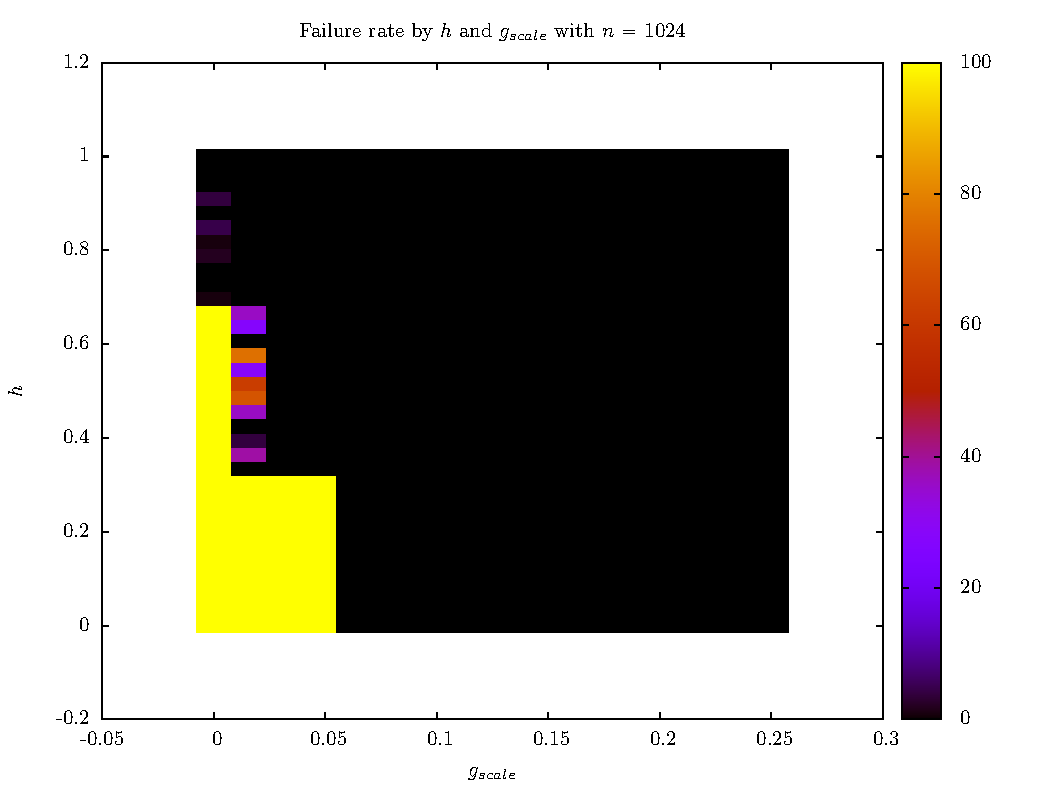
\includegraphics[width=\textwidth]{graphs/Annealing/annealing1024percent.pdf}
\caption{Failure rate of Annealing Sort with $n = 1024$}
\label{fig:Annealing:percent1024}
\end{figure}

\begin{figure}
\center
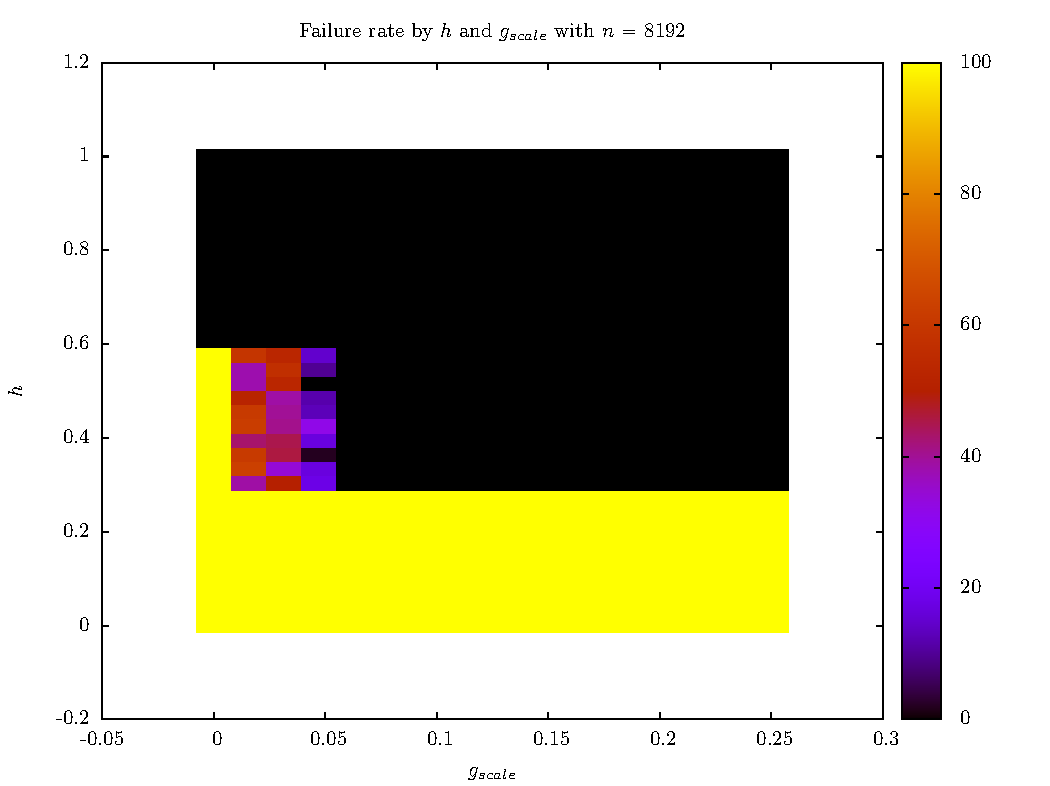
\includegraphics[width=\textwidth]{graphs/Annealing/annealing8192percent.pdf}
\caption{Failure rate of Annealing Sort with  $n = 8192$}
\label{fig:Annealing:percent8192}
\end{figure}

\subsection{Running Time}

Having investigated how failure rate depended on $h$ and $g_{scale}$, let us consider their effect on running time. Figure~\ref{fig:Annealing:time1024} and~\ref{fig:Annealing:time8192} show a map of running time with varying values of $h$ and $g_{scale}$.

From these maps we see that running time is clearly dominated by the contributions on the last phase, and the lower we scale its length, the better the running time. In fact, for both data sizes, it is almost impossible to spot the minor impact of increasing $h$, but it should be noted that it is definitely there, just rather minor compared to the great effect of $g_{scale}$.

\begin{figure}
\center
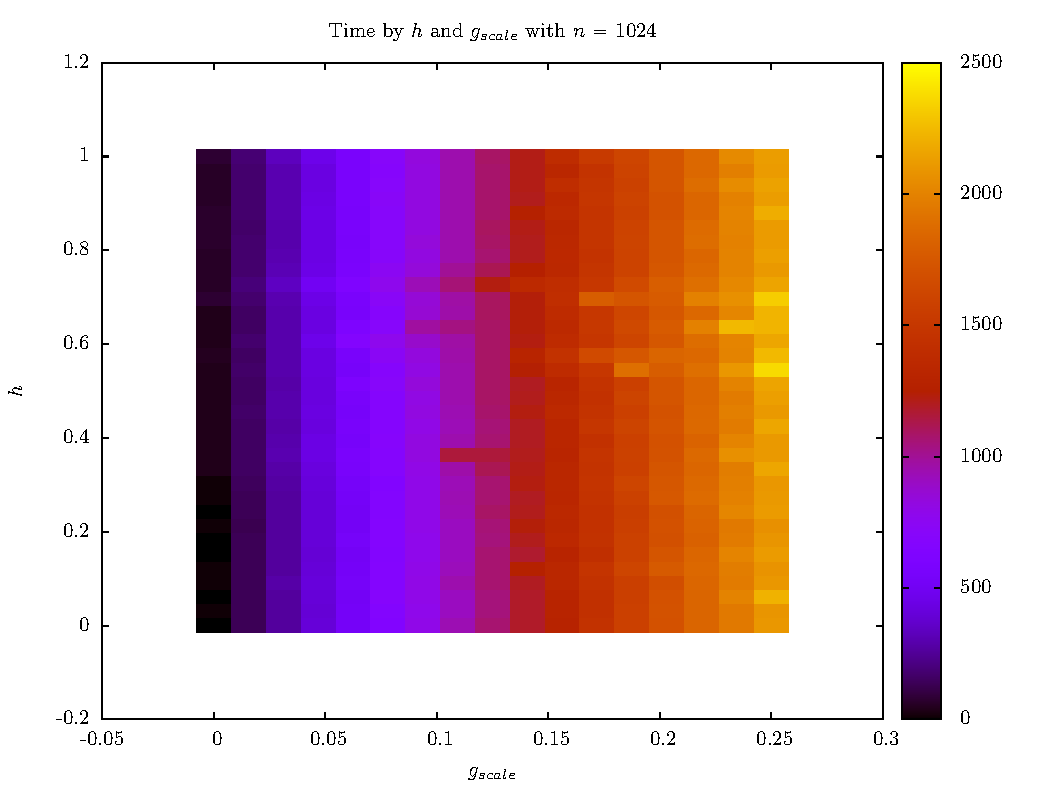
\includegraphics[width=\textwidth]{graphs/Annealing/annealing1024time.pdf}
\caption{Running time of Annealing Sort with  $n = 1024$}
\label{fig:Annealing:time1024}
\end{figure}

\begin{figure}
\center
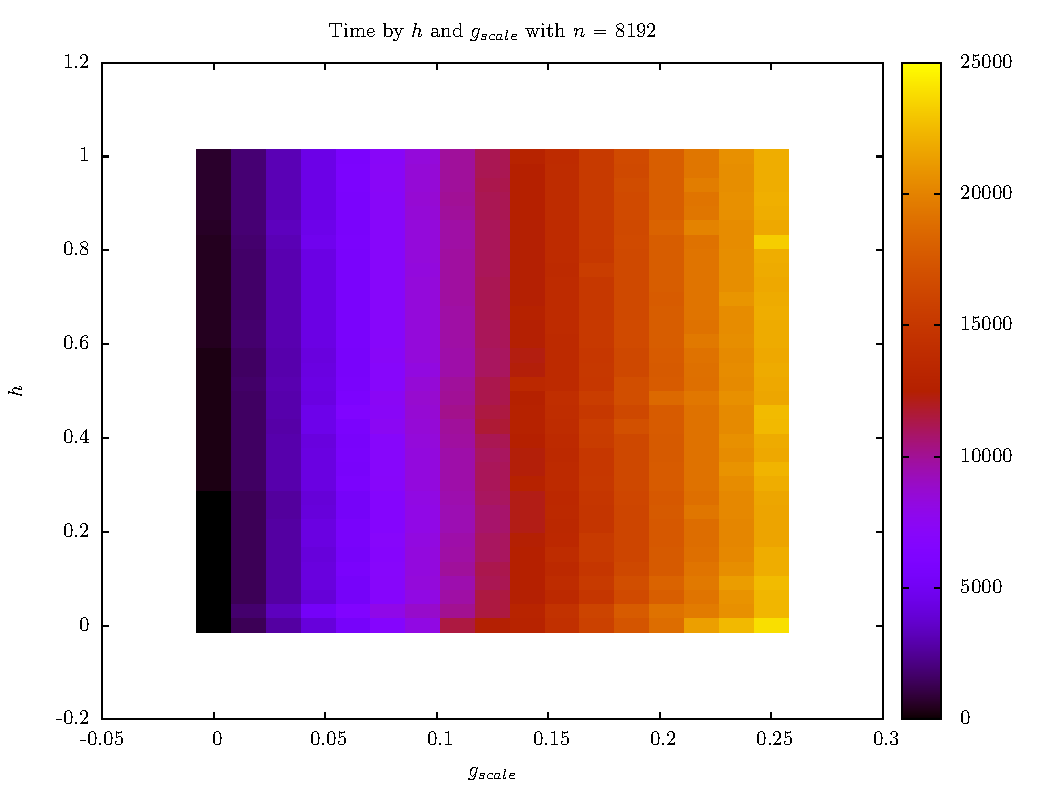
\includegraphics[width=\textwidth]{graphs/Annealing/annealing8192time.pdf}
\caption{Running time of Annealing Sort with $n = 8192$}
\label{fig:Annealing:time8192}
\end{figure}

\subsection{Large $n$}

From the previous experiments we learn two important lessons about the parameters used in constructing the annealing sequence for Annealing Sort;

\begin{enumerate}
\item Keep $h$ high, for a low dependable failure rate.
\item Keep $g_{scale}$ low, for a faster running time.
\end{enumerate}

Using this knowledge, we find the values of $h = 1$ and $g_{scale} = 0$ to be likely candidates for a speedy, reliable version of Annealing Sort.
In order to verify that these values does indeed sort with a high probability, tests were done using these parameters, and large values of $n$, which gave the following results:

\begin{table}[!ht]
\begin{adjustwidth}{-.5in}{-.5in}
\centering
\begin{tabular}{|l|c|c|c|c|c|c|c|c|c|c|c|}
\hline
n      & 1024 & 2048 & 4096 & 8192 & 16384 & 32768 & 65536 & 131072 & 262144 & 524288 & 1048576 \\ \hline
errors & 0    & 0    & 0    & 0    & 0     & 0     & 0     & 0      & 0      & 0      & 0       \\ \hline
\end{tabular}
\caption{Annealing Sort errors for large $n$, from 100 runs}
\end{adjustwidth}
\end{table}

From these results, we assume that these parameters are sufficient in providing a low failure rate, and their use in other experiments can be accepted.

\subsection{Experiment Results}

The experiment shows that using different parameters for Annealing Sort than those suggested in~\citeA{AnnealingSort} can improve the performance of the algorithm without negatively affecting the failure rate. 
This makes for a much faster version of Annealing Sort for use in practical applications.